
% Default to the notebook output style

    


% Inherit from the specified cell style.




    
\documentclass[11pt]{jsarticle}

    
    
    \usepackage[T1]{fontenc}
    % Nicer default font (+ math font) than Computer Modern for most use cases
    \usepackage{mathpazo}

    % Basic figure setup, for now with no caption control since it's done
    % automatically by Pandoc (which extracts ![](path) syntax from Markdown).
    \usepackage[dvipdfmx]{graphicx}
    % We will generate all images so they have a width \maxwidth. This means
    % that they will get their normal width if they fit onto the page, but
    % are scaled down if they would overflow the margins.

    %\makeatletter
    %\def\maxwidth{\ifdim\Gin@nat@width>\linewidth\linewidth
    %\else\Gin@nat@width\fi}
    %\makeatother
    %\let\Oldincludegraphics\includegraphics
    % Set max figure width to be 80% of text width, for now hardcoded.
    %\renewcommand{\includegraphics}[1]{\Oldincludegraphics[width=.8\maxwidth]{#1}}
    % Ensure that by default, figures have no caption (until we provide a
    % proper Figure object with a Caption API and a way to capture that
    % in the conversion process - todo).
    \usepackage{caption}
    \DeclareCaptionLabelFormat{nolabel}{}
    \captionsetup{labelformat=nolabel}

    \usepackage{adjustbox} % Used to constrain images to a maximum size 
    \usepackage{xcolor} % Allow colors to be defined
    \usepackage{enumerate} % Needed for markdown enumerations to work
    \usepackage{geometry} % Used to adjust the document margins
    \usepackage{amsmath} % Equations
    \usepackage{amssymb} % Equations
    \usepackage{textcomp} % defines textquotesingle
    % Hack from http://tex.stackexchange.com/a/47451/13684:
    \AtBeginDocument{%
        \def\PYZsq{\textquotesingle}% Upright quotes in Pygmentized code
    }
    \usepackage{upquote} % Upright quotes for verbatim code
    \usepackage{eurosym} % defines \euro
    \usepackage[mathletters]{ucs} % Extended unicode (utf-8) support
    \usepackage[utf8x]{inputenc} % Allow utf-8 characters in the tex document
    \usepackage{fancyvrb} % verbatim replacement that allows latex
    \usepackage{grffile} % extends the file name processing of package graphics 
                         % to support a larger range 
    % The hyperref package gives us a pdf with properly built
    % internal navigation ('pdf bookmarks' for the table of contents,
    % internal cross-reference links, web links for URLs, etc.)
    \usepackage{hyperref}
    \usepackage{longtable} % longtable support required by pandoc >1.10
    \usepackage{booktabs}  % table support for pandoc > 1.12.2
    \usepackage[inline]{enumitem} % IRkernel/repr support (it uses the enumerate* environment)
    \usepackage[normalem]{ulem} % ulem is needed to support strikethroughs (\sout)
                                % normalem makes italics be italics, not underlines
    

    
    
    % Colors for the hyperref package
    \definecolor{urlcolor}{rgb}{0,.145,.698}
    \definecolor{linkcolor}{rgb}{.71,0.21,0.01}
    \definecolor{citecolor}{rgb}{.12,.54,.11}

    % ANSI colors
    \definecolor{ansi-black}{HTML}{3E424D}
    \definecolor{ansi-black-intense}{HTML}{282C36}
    \definecolor{ansi-red}{HTML}{E75C58}
    \definecolor{ansi-red-intense}{HTML}{B22B31}
    \definecolor{ansi-green}{HTML}{00A250}
    \definecolor{ansi-green-intense}{HTML}{007427}
    \definecolor{ansi-yellow}{HTML}{DDB62B}
    \definecolor{ansi-yellow-intense}{HTML}{B27D12}
    \definecolor{ansi-blue}{HTML}{208FFB}
    \definecolor{ansi-blue-intense}{HTML}{0065CA}
    \definecolor{ansi-magenta}{HTML}{D160C4}
    \definecolor{ansi-magenta-intense}{HTML}{A03196}
    \definecolor{ansi-cyan}{HTML}{60C6C8}
    \definecolor{ansi-cyan-intense}{HTML}{258F8F}
    \definecolor{ansi-white}{HTML}{C5C1B4}
    \definecolor{ansi-white-intense}{HTML}{A1A6B2}

    % commands and environments needed by pandoc snippets
    % extracted from the output of `pandoc -s`
    \providecommand{\tightlist}{%
      \setlength{\itemsep}{0pt}\setlength{\parskip}{0pt}}
    \DefineVerbatimEnvironment{Highlighting}{Verbatim}{commandchars=\\\{\}}
    % Add ',fontsize=\small' for more characters per line
    \newenvironment{Shaded}{}{}
    \newcommand{\KeywordTok}[1]{\textcolor[rgb]{0.00,0.44,0.13}{\textbf{{#1}}}}
    \newcommand{\DataTypeTok}[1]{\textcolor[rgb]{0.56,0.13,0.00}{{#1}}}
    \newcommand{\DecValTok}[1]{\textcolor[rgb]{0.25,0.63,0.44}{{#1}}}
    \newcommand{\BaseNTok}[1]{\textcolor[rgb]{0.25,0.63,0.44}{{#1}}}
    \newcommand{\FloatTok}[1]{\textcolor[rgb]{0.25,0.63,0.44}{{#1}}}
    \newcommand{\CharTok}[1]{\textcolor[rgb]{0.25,0.44,0.63}{{#1}}}
    \newcommand{\StringTok}[1]{\textcolor[rgb]{0.25,0.44,0.63}{{#1}}}
    \newcommand{\CommentTok}[1]{\textcolor[rgb]{0.38,0.63,0.69}{\textit{{#1}}}}
    \newcommand{\OtherTok}[1]{\textcolor[rgb]{0.00,0.44,0.13}{{#1}}}
    \newcommand{\AlertTok}[1]{\textcolor[rgb]{1.00,0.00,0.00}{\textbf{{#1}}}}
    \newcommand{\FunctionTok}[1]{\textcolor[rgb]{0.02,0.16,0.49}{{#1}}}
    \newcommand{\RegionMarkerTok}[1]{{#1}}
    \newcommand{\ErrorTok}[1]{\textcolor[rgb]{1.00,0.00,0.00}{\textbf{{#1}}}}
    \newcommand{\NormalTok}[1]{{#1}}
    
    % Additional commands for more recent versions of Pandoc
    \newcommand{\ConstantTok}[1]{\textcolor[rgb]{0.53,0.00,0.00}{{#1}}}
    \newcommand{\SpecialCharTok}[1]{\textcolor[rgb]{0.25,0.44,0.63}{{#1}}}
    \newcommand{\VerbatimStringTok}[1]{\textcolor[rgb]{0.25,0.44,0.63}{{#1}}}
    \newcommand{\SpecialStringTok}[1]{\textcolor[rgb]{0.73,0.40,0.53}{{#1}}}
    \newcommand{\ImportTok}[1]{{#1}}
    \newcommand{\DocumentationTok}[1]{\textcolor[rgb]{0.73,0.13,0.13}{\textit{{#1}}}}
    \newcommand{\AnnotationTok}[1]{\textcolor[rgb]{0.38,0.63,0.69}{\textbf{\textit{{#1}}}}}
    \newcommand{\CommentVarTok}[1]{\textcolor[rgb]{0.38,0.63,0.69}{\textbf{\textit{{#1}}}}}
    \newcommand{\VariableTok}[1]{\textcolor[rgb]{0.10,0.09,0.49}{{#1}}}
    \newcommand{\ControlFlowTok}[1]{\textcolor[rgb]{0.00,0.44,0.13}{\textbf{{#1}}}}
    \newcommand{\OperatorTok}[1]{\textcolor[rgb]{0.40,0.40,0.40}{{#1}}}
    \newcommand{\BuiltInTok}[1]{{#1}}
    \newcommand{\ExtensionTok}[1]{{#1}}
    \newcommand{\PreprocessorTok}[1]{\textcolor[rgb]{0.74,0.48,0.00}{{#1}}}
    \newcommand{\AttributeTok}[1]{\textcolor[rgb]{0.49,0.56,0.16}{{#1}}}
    \newcommand{\InformationTok}[1]{\textcolor[rgb]{0.38,0.63,0.69}{\textbf{\textit{{#1}}}}}
    \newcommand{\WarningTok}[1]{\textcolor[rgb]{0.38,0.63,0.69}{\textbf{\textit{{#1}}}}}
    
    
    % Define a nice break command that doesn't care if a line doesn't already
    % exist.
    \def\br{\hspace*{\fill} \\* }
    % Math Jax compatability definitions
    \def\gt{>}
    \def\lt{<}
    % Document parameters
    \title{GCI Final Report}
    
    
    

    % Pygments definitions
    
\makeatletter
\def\PY@reset{\let\PY@it=\relax \let\PY@bf=\relax%
    \let\PY@ul=\relax \let\PY@tc=\relax%
    \let\PY@bc=\relax \let\PY@ff=\relax}
\def\PY@tok#1{\csname PY@tok@#1\endcsname}
\def\PY@toks#1+{\ifx\relax#1\empty\else%
    \PY@tok{#1}\expandafter\PY@toks\fi}
\def\PY@do#1{\PY@bc{\PY@tc{\PY@ul{%
    \PY@it{\PY@bf{\PY@ff{#1}}}}}}}
\def\PY#1#2{\PY@reset\PY@toks#1+\relax+\PY@do{#2}}

\expandafter\def\csname PY@tok@w\endcsname{\def\PY@tc##1{\textcolor[rgb]{0.73,0.73,0.73}{##1}}}
\expandafter\def\csname PY@tok@c\endcsname{\let\PY@it=\textit\def\PY@tc##1{\textcolor[rgb]{0.25,0.50,0.50}{##1}}}
\expandafter\def\csname PY@tok@cp\endcsname{\def\PY@tc##1{\textcolor[rgb]{0.74,0.48,0.00}{##1}}}
\expandafter\def\csname PY@tok@k\endcsname{\let\PY@bf=\textbf\def\PY@tc##1{\textcolor[rgb]{0.00,0.50,0.00}{##1}}}
\expandafter\def\csname PY@tok@kp\endcsname{\def\PY@tc##1{\textcolor[rgb]{0.00,0.50,0.00}{##1}}}
\expandafter\def\csname PY@tok@kt\endcsname{\def\PY@tc##1{\textcolor[rgb]{0.69,0.00,0.25}{##1}}}
\expandafter\def\csname PY@tok@o\endcsname{\def\PY@tc##1{\textcolor[rgb]{0.40,0.40,0.40}{##1}}}
\expandafter\def\csname PY@tok@ow\endcsname{\let\PY@bf=\textbf\def\PY@tc##1{\textcolor[rgb]{0.67,0.13,1.00}{##1}}}
\expandafter\def\csname PY@tok@nb\endcsname{\def\PY@tc##1{\textcolor[rgb]{0.00,0.50,0.00}{##1}}}
\expandafter\def\csname PY@tok@nf\endcsname{\def\PY@tc##1{\textcolor[rgb]{0.00,0.00,1.00}{##1}}}
\expandafter\def\csname PY@tok@nc\endcsname{\let\PY@bf=\textbf\def\PY@tc##1{\textcolor[rgb]{0.00,0.00,1.00}{##1}}}
\expandafter\def\csname PY@tok@nn\endcsname{\let\PY@bf=\textbf\def\PY@tc##1{\textcolor[rgb]{0.00,0.00,1.00}{##1}}}
\expandafter\def\csname PY@tok@ne\endcsname{\let\PY@bf=\textbf\def\PY@tc##1{\textcolor[rgb]{0.82,0.25,0.23}{##1}}}
\expandafter\def\csname PY@tok@nv\endcsname{\def\PY@tc##1{\textcolor[rgb]{0.10,0.09,0.49}{##1}}}
\expandafter\def\csname PY@tok@no\endcsname{\def\PY@tc##1{\textcolor[rgb]{0.53,0.00,0.00}{##1}}}
\expandafter\def\csname PY@tok@nl\endcsname{\def\PY@tc##1{\textcolor[rgb]{0.63,0.63,0.00}{##1}}}
\expandafter\def\csname PY@tok@ni\endcsname{\let\PY@bf=\textbf\def\PY@tc##1{\textcolor[rgb]{0.60,0.60,0.60}{##1}}}
\expandafter\def\csname PY@tok@na\endcsname{\def\PY@tc##1{\textcolor[rgb]{0.49,0.56,0.16}{##1}}}
\expandafter\def\csname PY@tok@nt\endcsname{\let\PY@bf=\textbf\def\PY@tc##1{\textcolor[rgb]{0.00,0.50,0.00}{##1}}}
\expandafter\def\csname PY@tok@nd\endcsname{\def\PY@tc##1{\textcolor[rgb]{0.67,0.13,1.00}{##1}}}
\expandafter\def\csname PY@tok@s\endcsname{\def\PY@tc##1{\textcolor[rgb]{0.73,0.13,0.13}{##1}}}
\expandafter\def\csname PY@tok@sd\endcsname{\let\PY@it=\textit\def\PY@tc##1{\textcolor[rgb]{0.73,0.13,0.13}{##1}}}
\expandafter\def\csname PY@tok@si\endcsname{\let\PY@bf=\textbf\def\PY@tc##1{\textcolor[rgb]{0.73,0.40,0.53}{##1}}}
\expandafter\def\csname PY@tok@se\endcsname{\let\PY@bf=\textbf\def\PY@tc##1{\textcolor[rgb]{0.73,0.40,0.13}{##1}}}
\expandafter\def\csname PY@tok@sr\endcsname{\def\PY@tc##1{\textcolor[rgb]{0.73,0.40,0.53}{##1}}}
\expandafter\def\csname PY@tok@ss\endcsname{\def\PY@tc##1{\textcolor[rgb]{0.10,0.09,0.49}{##1}}}
\expandafter\def\csname PY@tok@sx\endcsname{\def\PY@tc##1{\textcolor[rgb]{0.00,0.50,0.00}{##1}}}
\expandafter\def\csname PY@tok@m\endcsname{\def\PY@tc##1{\textcolor[rgb]{0.40,0.40,0.40}{##1}}}
\expandafter\def\csname PY@tok@gh\endcsname{\let\PY@bf=\textbf\def\PY@tc##1{\textcolor[rgb]{0.00,0.00,0.50}{##1}}}
\expandafter\def\csname PY@tok@gu\endcsname{\let\PY@bf=\textbf\def\PY@tc##1{\textcolor[rgb]{0.50,0.00,0.50}{##1}}}
\expandafter\def\csname PY@tok@gd\endcsname{\def\PY@tc##1{\textcolor[rgb]{0.63,0.00,0.00}{##1}}}
\expandafter\def\csname PY@tok@gi\endcsname{\def\PY@tc##1{\textcolor[rgb]{0.00,0.63,0.00}{##1}}}
\expandafter\def\csname PY@tok@gr\endcsname{\def\PY@tc##1{\textcolor[rgb]{1.00,0.00,0.00}{##1}}}
\expandafter\def\csname PY@tok@ge\endcsname{\let\PY@it=\textit}
\expandafter\def\csname PY@tok@gs\endcsname{\let\PY@bf=\textbf}
\expandafter\def\csname PY@tok@gp\endcsname{\let\PY@bf=\textbf\def\PY@tc##1{\textcolor[rgb]{0.00,0.00,0.50}{##1}}}
\expandafter\def\csname PY@tok@go\endcsname{\def\PY@tc##1{\textcolor[rgb]{0.53,0.53,0.53}{##1}}}
\expandafter\def\csname PY@tok@gt\endcsname{\def\PY@tc##1{\textcolor[rgb]{0.00,0.27,0.87}{##1}}}
\expandafter\def\csname PY@tok@err\endcsname{\def\PY@bc##1{\setlength{\fboxsep}{0pt}\fcolorbox[rgb]{1.00,0.00,0.00}{1,1,1}{\strut ##1}}}
\expandafter\def\csname PY@tok@kc\endcsname{\let\PY@bf=\textbf\def\PY@tc##1{\textcolor[rgb]{0.00,0.50,0.00}{##1}}}
\expandafter\def\csname PY@tok@kd\endcsname{\let\PY@bf=\textbf\def\PY@tc##1{\textcolor[rgb]{0.00,0.50,0.00}{##1}}}
\expandafter\def\csname PY@tok@kn\endcsname{\let\PY@bf=\textbf\def\PY@tc##1{\textcolor[rgb]{0.00,0.50,0.00}{##1}}}
\expandafter\def\csname PY@tok@kr\endcsname{\let\PY@bf=\textbf\def\PY@tc##1{\textcolor[rgb]{0.00,0.50,0.00}{##1}}}
\expandafter\def\csname PY@tok@bp\endcsname{\def\PY@tc##1{\textcolor[rgb]{0.00,0.50,0.00}{##1}}}
\expandafter\def\csname PY@tok@fm\endcsname{\def\PY@tc##1{\textcolor[rgb]{0.00,0.00,1.00}{##1}}}
\expandafter\def\csname PY@tok@vc\endcsname{\def\PY@tc##1{\textcolor[rgb]{0.10,0.09,0.49}{##1}}}
\expandafter\def\csname PY@tok@vg\endcsname{\def\PY@tc##1{\textcolor[rgb]{0.10,0.09,0.49}{##1}}}
\expandafter\def\csname PY@tok@vi\endcsname{\def\PY@tc##1{\textcolor[rgb]{0.10,0.09,0.49}{##1}}}
\expandafter\def\csname PY@tok@vm\endcsname{\def\PY@tc##1{\textcolor[rgb]{0.10,0.09,0.49}{##1}}}
\expandafter\def\csname PY@tok@sa\endcsname{\def\PY@tc##1{\textcolor[rgb]{0.73,0.13,0.13}{##1}}}
\expandafter\def\csname PY@tok@sb\endcsname{\def\PY@tc##1{\textcolor[rgb]{0.73,0.13,0.13}{##1}}}
\expandafter\def\csname PY@tok@sc\endcsname{\def\PY@tc##1{\textcolor[rgb]{0.73,0.13,0.13}{##1}}}
\expandafter\def\csname PY@tok@dl\endcsname{\def\PY@tc##1{\textcolor[rgb]{0.73,0.13,0.13}{##1}}}
\expandafter\def\csname PY@tok@s2\endcsname{\def\PY@tc##1{\textcolor[rgb]{0.73,0.13,0.13}{##1}}}
\expandafter\def\csname PY@tok@sh\endcsname{\def\PY@tc##1{\textcolor[rgb]{0.73,0.13,0.13}{##1}}}
\expandafter\def\csname PY@tok@s1\endcsname{\def\PY@tc##1{\textcolor[rgb]{0.73,0.13,0.13}{##1}}}
\expandafter\def\csname PY@tok@mb\endcsname{\def\PY@tc##1{\textcolor[rgb]{0.40,0.40,0.40}{##1}}}
\expandafter\def\csname PY@tok@mf\endcsname{\def\PY@tc##1{\textcolor[rgb]{0.40,0.40,0.40}{##1}}}
\expandafter\def\csname PY@tok@mh\endcsname{\def\PY@tc##1{\textcolor[rgb]{0.40,0.40,0.40}{##1}}}
\expandafter\def\csname PY@tok@mi\endcsname{\def\PY@tc##1{\textcolor[rgb]{0.40,0.40,0.40}{##1}}}
\expandafter\def\csname PY@tok@il\endcsname{\def\PY@tc##1{\textcolor[rgb]{0.40,0.40,0.40}{##1}}}
\expandafter\def\csname PY@tok@mo\endcsname{\def\PY@tc##1{\textcolor[rgb]{0.40,0.40,0.40}{##1}}}
\expandafter\def\csname PY@tok@ch\endcsname{\let\PY@it=\textit\def\PY@tc##1{\textcolor[rgb]{0.25,0.50,0.50}{##1}}}
\expandafter\def\csname PY@tok@cm\endcsname{\let\PY@it=\textit\def\PY@tc##1{\textcolor[rgb]{0.25,0.50,0.50}{##1}}}
\expandafter\def\csname PY@tok@cpf\endcsname{\let\PY@it=\textit\def\PY@tc##1{\textcolor[rgb]{0.25,0.50,0.50}{##1}}}
\expandafter\def\csname PY@tok@c1\endcsname{\let\PY@it=\textit\def\PY@tc##1{\textcolor[rgb]{0.25,0.50,0.50}{##1}}}
\expandafter\def\csname PY@tok@cs\endcsname{\let\PY@it=\textit\def\PY@tc##1{\textcolor[rgb]{0.25,0.50,0.50}{##1}}}

\def\PYZbs{\char`\\}
\def\PYZus{\char`\_}
\def\PYZob{\char`\{}
\def\PYZcb{\char`\}}
\def\PYZca{\char`\^}
\def\PYZam{\char`\&}
\def\PYZlt{\char`\<}
\def\PYZgt{\char`\>}
\def\PYZsh{\char`\#}
\def\PYZpc{\char`\%}
\def\PYZdl{\char`\$}
\def\PYZhy{\char`\-}
\def\PYZsq{\char`\'}
\def\PYZdq{\char`\"}
\def\PYZti{\char`\~}
% for compatibility with earlier versions
\def\PYZat{@}
\def\PYZlb{[}
\def\PYZrb{]}
\makeatother


    % Exact colors from NB
    \definecolor{incolor}{rgb}{0.0, 0.0, 0.5}
    \definecolor{outcolor}{rgb}{0.545, 0.0, 0.0}



    
    % Prevent overflowing lines due to hard-to-break entities
    \sloppy 
    % Setup hyperref package
    \hypersetup{
      breaklinks=true,  % so long urls are correctly broken across lines
      colorlinks=true,
      urlcolor=urlcolor,
      linkcolor=linkcolor,
      citecolor=citecolor,
      }
    % Slightly bigger margins than the latex defaults
    
    \geometry{verbose,tmargin=1in,bmargin=1in,lmargin=1in,rmargin=1in}
    
    
    \author{工学系研究科航空宇宙専攻修士一年\\荒居 秀尚}

    \begin{document}
    
    
    \maketitle
    
    

    \begin{abstract}
本稿は、現在Kaggleにおいて行われているHome Credit GroupのDefault Riskを評価するコンペティションHome-Credit-Default-Riskに絡めて
Home Creditグループにとってより価値の高いクレジットスコアリングモデルを提案するものである。本稿は、背景・導入、仮説・評価、価値提案の3つのセクションから構成される。最初に背景・導入の章においては、クレジットスコアリングモデルの意義やその歴史的背景、そして現在における構築の手順と構築にまつわる課題を提示する。続く仮説・評価の章においてはHome Credot Groupにおけるクレジットスコアリングモデル構築の取り組みやHome Credit Groupが抱えている課題、Home Credit GroupがKaggleのコンペティションに主催者として参加するに至った経緯に関して断片的な情報から仮説構築を試み、その課題を解決するモデルの構築を行う。また、そのモデルを仮説に基づいて選択された評価手段によって評価する。最後の価値提案の章においては提案するモデルが持つ価値をHome Credit Groupにもたらす影響から概算し、既存の信用機関におけるクレジットスコアリングモデルの構築の費用などを参照したうえで価格提示を行う。
\end{abstract}
    \section{背景・導入}\label{ux80ccux666fux5c0eux5165}

\subsection{クレジットスコアリングの意義}\label{ux30afux30ecux30b8ux30c3ux30c8ux30b9ux30b3ux30a2ux30eaux30f3ux30b0ux306eux610fux7fa9}
銀行や信用機関における信用リスク管理業務は単なる貸出審査の効率化以上の意義があると考えられる。貸出業務は金融機関の業務の中でも大きな割合を占めるが、そこで重視されるのはリスクとリターンのバランスである。貸出にあたっての不確定性が大きく完全な資金回収を行うことができないことは大きな痛手となる一方で、確実性を求めて一部の優良な取引相手や確実な資金回収が見込まれる相手だけと取引をすることは、銀行・金融機関の利益にあまりつながらない。したがってその中間をとり、リスクとリターンがバランスするような点において取引をするか/しないかを定めるのは非常に重要と言える。この決定は一般には銀行・金融機関のリスク選好性によって変わるものであるが、その決定に大きな影響を及ぼすのが信用リスク管理である。\\

信用リスクの管理は「貸出資産の損失可能性を事前に推算すること」と言い換えることもできるが\cite{risk-management}、これにより貸出資産の価値を評価することができ、金融機関それ自体の健康状態を管理することができるともいえる。金融機関の健康状態の悪化はしばしば経済的な不安要因となり社会を大きく揺るがすことにもつながりかねない。近年では、米国に端を発した信用危機が世界的な経済不安を引き起こすなどの例もあったが、これも信用リスク管理の失敗によるものであり、この業務の重要性を端的に表した一例と言える。
    クレジットスコアリングは上記のような信用リスク管理業務のなかでも大きな重要度を持った業務である。信用リスクの推算は貸出を行った場合の予想損失(EL)の推算とも言い換えられるが、予想損失の構成パラメータは、デフォルト時貸出残高(EAD)、デフォルト率(PD)、デフォルト時損失率(LGD)の積として表される。式として表すと
\[
  EL = EAD \times PD \times LGD
\]
となる。このうちクレジットスコアリングが行うのはデフォルト率(PD)の推算である。この推算を誤ると、実際には大きなリスクを抱えている案件のリスクを過小評価してしまったり実際には優良な債務者に対して貸出を行わない、といった意思決定に繋がる恐れがあり非常に重要である。

    \subsection{クレジットスコアリングの歴史的背景}\label{ux30afux30ecux30b8ux30c3ux30c8ux30b9ux30b3ux30a2ux30eaux30f3ux30b0ux306eux6b74ux53f2ux7684ux80ccux666f}
クレジットスコアリング自体の登場は非常に古く、1950年代に開発され始め1960年代に実用化されたと言われている\cite{perspective}。これらは、登場当初は上述のような理由は主ではなくどちらかといえば現場の負担を軽減する目的で導入されたと言われているがその後急速に普及した。\\

米国では過去数十年にわたってクレジットスコアリングが消費者の生活の非常に大きな部分を占めてきた経緯がある。クレジットスコアが生活に影響を与える範囲は広く、元々はローンの貸出などの指標として用いられていたものの、住宅の入居判断や就職などにおいてもクレジットスコアの良し悪しが関わってくるようになり現在では生活の多くの部分を支配し格差を固定化する要因の一つとなっているとも言われる。米国で普及するクレジットスコアリングは大きく3つの企業による指標が用いられることが多い。その3企業はTransUnion、Equifax、ExperianであるがこれらはFICOスコアという指標の計算方法をベースに独自のクレジットスコアの算出をしている\cite{annuity}が大まかには以下のような内訳であると言われている。
    \begin{itemize}
\tightlist
\item
  35\%が過去の支払い履歴
\item
  30\%が現在の負債
\item
  15\%が信用履歴の長さ
\item
  10\%が最近の融資問い合わせ額
\item
  10\%がアカウントの種類/個数
\end{itemize}

また、クレジットスコアを改善させるためのベストプラクティスといったものもよく伝え聞かれており以下のようなものが挙げられている。

\begin{itemize}
\tightlist
\item
  クレジット限度額の65\%-75\%には手をつけないようにすること。多すぎるとリスクになり、少なすぎると信用機関にとって良くわからない人になる。
\item
  昔のアカウントをcloseしないでopenなままにしておくこと、誘惑に負けてしまいそうならカードを捨てなさい。
\item
  新規アカウント開設は控えめに。企業や貸し手が信用情報を参照するたびにクレジットスコアは下がります。
\item
  延滞や延滞期限をできるだけ残さないようにすること。
\item
  安易な解決策に飛びつかないように。詐欺の場合もあります。
\end{itemize}

    \subsection{現在における構築の手順・課題}\label{ux73feux5728ux306bux304aux3051ux308bux69cbux7bc9ux306eux624bux9806ux8ab2ux984c}

    クレジットスコアリングモデルは各金融機関の生命線であるため具体的なアルゴリズムや説明変数が公開されている例はあまり存在せず、断片的な情報を組み合わせて推測する必要がある。また、信用機関は目的に応じて複数のクレジットスコアリングモデルを使い分けていると考えられるため\cite{fujitsu}、よく用いられていると考えられる手法をその背景などに着目しながら紹介する。また、クレジットスコアリングに用いられる説明変数はその国や地域における法規や産業構造の違いなどから異なる可能性が示唆される\cite{kirill}。

    \subsubsection{クレジットスコアリングの手法}\label{ux30afux30ecux30b8ux30c3ux30c8ux30b9ux30b3ux30a2ux30eaux30f3ux30b0ux306eux624bux6cd5}

    現在のクレジットスコアリングはその用例に応じて複数の手法を使い分ける試みがなされていると考えられる\cite{fujitsu}。以下はそれらについてと、その用法に関しての説明である。

\begin{itemize}
\tightlist
\item
  スコアカード
\end{itemize}

経験的な指標に基づきある条件を満たしているときは点数を加算することで、合計点数をクレジットスコアとするモデルである。例としては、勤続年数1年未満は10点、1-3年は30点、3-10年は50点、10年以上は70点と言った具合である\cite{scorecard}。非常に単純な指標であるため理解は容易であるが、経験的な指標であるため意思決定の際の強い根拠とするには弱く、また現実の複雑な状況に即した判断にも使いづらいという難点が存在する。

\begin{itemize}
\tightlist
\item
  判別分析
\end{itemize}

線形分離モデルを用いてデフォルト先と非デフォルト先をより良く区分する線を決定する手法である。線形手法であるため、複雑な境界を表現できないという点で現実の複雑な状況に即した判断には使いづらく、直感的な理解もスコアカードに比べると容易ではない。そのため、意思決定の際にも強い根拠として用いることが難しい。

\begin{itemize}
\tightlist
\item
  ロジスティック回帰
\end{itemize}

一般化線形モデルを用いてデフォルト確率を推算することができるため、意思決定においては使いやすい。一方で、表現力は線形判別分析とおよそ同程度である。直感的な理解のしやすさも判別分析と同程度と言える。

\begin{itemize}
\tightlist
\item
  決定木
\end{itemize}

確率の推算にも用いることができるため意思決定においては使いやすい。非線形の決定境界を表現できる一方、過学習しやすいという欠点もあり複雑な状況に即した判断にはやや使いづらい。一方、判断の根拠を階層的な分岐で表現でき理解のしやすさは判別分析やロジスティック回帰よりよいといえる。

\begin{itemize}
\tightlist
\item
  ニューラルネット
\end{itemize}

中間層の複雑さを増すことでより複雑な境界を表現できる一方で、説明性に劣る面があるため、意思決定においても使いづらいという側面が存在する。

\begin{itemize}
\tightlist
\item
  カーネルSVM
\end{itemize}

カーネル関数を用いて高次元空間に特徴を写したうえで線形分離をする手法で、数年前までニューラルネット以上の成績を出すと言われていた一方、説明性に劣るため、意思決定の場では使いづらいという側面がある。

\begin{itemize}
\tightlist
\item
  アンサンブル手法
\end{itemize}

勾配ブースティングやニューラルネットと決定木のブレンディング・スタッキングなど、近年Kaggleなどのコンペティションにおいても隆盛を誇っている手法である。シングルモデル以上の成績を示すこともある一方で説明性は低く意思決定の場で決定打とはならないという現状があると考えられる。

    \subsubsection{説明変数について}\label{ux8aacux660eux5909ux6570ux306bux3064ux3044ux3066}
説明変数の選択に関しては、スコアリングの具体的なアルゴリズム以上に企業の秘密に関わるため、公開されている例はないが断片的な情報からおおよそどの企業も用いていそうな説明変数の推測は可能である。一方、その他の部分は企業ごとのスコアリングにおいて大きな特徴となりうる一方で推測は難しくその個数もスコアリングを行う企業によって異なることが予想される。説明変数の選択についてもアルゴリズムの選択同様、用途によって分けていると考えられるため、参照できる資料をもとに考察を行う。\\

まず、説明変数の個数についてであるが、一般的に50以上になることはないようである\cite{kirill}\cite{perspective}。これは、説明変数の増大に伴いモデルの複雑さが増し、説明性の低下を招いたり保守管理のコストが増すといった側面があり、説明変数を増やすことによる表現力の向上との兼ね合いから考えてもこれ以上の数にはしづらいという背景が存在する。また、近年はビッグデータの活用などにより複雑なモデルに大量のデータを投入するようなPD推定の取り組みもあるものの、現状ではいくつかの"スマートに"加工された説明変数を用いることでPD推定を行う手法が主流であり、説明変数の個数のおおよその値としては9~50程度と見積もることができる\cite{kirill}\cite{mlit}。説明変数の種類に関しては、各種金融機関に対する国土交通省住宅局の2011年の調査に挙げられたものを参考とした\cite{mlit}。この調査では住宅ローン審査において金融機関が審査項目に入れることが多かった項目を項目別割合として結果にあげている。

\begin{table}[htbp]
\begin{center}
  \begin{tabular}{lr} \hline\hline
    審査項目 & 回答数の割合 \\ \hline\hline
    完済時年齢 & 91.90\% \\
    返済負担率 & 90.10\% \\
    借入時年齢 & 89.90\% \\
    勤続年数 & 88.50\% \\
    年収 & 88.10\% \\
    健康状態 & 88.10\% \\
    担保評価 & 85.90\% \\
    連帯保証 & 85.10\% \\
    債務状況・返済状況 & 84.90\% \\
    融資可能額(購入時) & 84.70\% \\
    融資可能額(借り入れ時) & 83.30\% \\
    金融機関の営業エリア & 80.20\% \\
    雇用形態 & 63.10\% \\
    申込人との取引状況 & 59.70\% \\
    国籍 & 47.60\% \\
    業種 & 40.20\% \\
    雇用先の規模 & 26.60\% \\
    家族構成 & 26.00\% \\
    所有資産 & 22.70\% \\
    性別 & 16.50\% \\
    その他 & 9.70\% \\
  \end{tabular}
  \caption{住宅ローン審査において民間金融機関が重視する項目}
\end{center}
\end{table}
また、\cite{stepwisebayse}などでは、変数選択により(1)「勤続年数」(2)「自己資本比率」(3)「合算年収倍率」(4)「借入期間」(5)「事業主フラグ」(6)「小企業フラグ」(7)「中企業フラグ」(8)「地域別CI成長率」(9)「地域別失業率」の9変数に絞ってPD推定を行っている。いずれにしても、生活基盤の安定性などを評価する指標(勤続年数・年収・雇用先規模・業種・健康状態など)、過去の信用情報履歴(債務状況・返済状況、自己資本比率)、将来性(完済時年齢、借入時年齢、借入期間)などを説明変数に取り入れている一方で、コンプライアンス上問題になりかねない説明変数(家族構成・性別・国籍など)は審査項目として使われづらい傾向があると考えられる。
    \subsubsection{金融機関の抱える課題}\label{ux91d1ux878dux6a5fux95a2ux306eux62b1ux3048ux308bux8ab2ux984c}

    クレジットスコアリングに関連して金融機関が抱える課題はいくつかに分けられる\cite{fujitsu}。

\begin{itemize}
\tightlist
\item
  モデルが複雑なため、作成過程や計算過程がブラックボックス化してしまう
\item
  モデルの精度に不安があり、モデルの見直しの必要がある
\item
  モデルの見直しのたびに、コンサルティングやシステム改修の費用がかかる
\end{itemize}

といったことが挙げられている。これらに関して金融機関により挙げられている対策は以下のようになる。

\begin{itemize}
\tightlist
\item
  研修の実施
\item
  運用目的にあわせて複雑さと説明性のトレードオフを考慮したモデルの再構築
\item
  最新の機械学習手法の利用
\item
  テンプレートの利用
\end{itemize}

また、この他に\cite{kirill}などに挙げられている、詐欺のリスクも大きな課題となっているようである。詐欺を試みる者は虚偽の申告をする場合も多く、データには現れづらいと考えられる。

    \section{仮説・評価}\label{ux4eeeux8aacux8a55ux4fa1}

\subsection{Home Credit
Groupにおけるクレジットスコアリングモデル構築の取り組み}\label{home-credit-groupux306bux304aux3051ux308bux30afux30ecux30b8ux30c3ux30c8ux30b9ux30b3ux30a2ux30eaux30f3ux30b0ux30e2ux30c7ux30ebux69cbux7bc9ux306eux53d6ux308aux7d44ux307f}

    Home Credit
GroupにおけるクレジットスコアリングはKaggleのコンペティションのディスカッションにおいて主催者であるKirill
Odintsov氏が語っている内容から部分的に推察できる\cite{kirill}。以下はそれらのディスカッションの内容を要約したものである。

\begin{itemize}
\tightlist
\item
  AUC
  0.77は現行のモデルよりはやや低いが抜かれるのは時間の問題である。それは、ビジネスにおける制約上用いることが出来ないデータを今回のコンペティションでは数多く用意しているからである。
\item
  Home Credit
  Groupにおいて用いられているモデルはロジスティック回帰や決定木などの単純なものもあるし、より高度なXGBなどの勾配ブースティング法やニューラルネットを使ったものも存在する。
\item
  既に多くの融資を受けている人にお金を貸すことは企業としては利益になると考えられるので積極的に行うべきことであるが、顧客を過剰に借金を抱えた状態にしてしまう可能性があるのでPDが小さいと予測されていたとしても避けたいことである。
\item
  100以上の特徴を加えてモニタリングするよりも、50くらいの特徴でやや低いくらいの精度を出せるほうが良い。
\item
  最終的にはより簡単なモデルを使うにしても一度は複雑なモデルを試すことを行っている。
\item
  モデルの再構築時には古いモデルを通ってきた母集団で学習を行うため、そこには含まれていなかったような人が新規申し込みをしたとして本来は落とされるべきであるにもかかわらず審査を通過してしまう可能性があり大きな問題となっている。
\item
  実際のモデルでは、性別・結婚状態・子供の数など、コンプライアンス的に使えない変数がある。
\item
  その時点での景気などの情報を使えば推論の精度は良くなるがそれは入れられない。
\item
  Home Credit
  Groupのデータサイエンスチームが用意しているモデルは多数ある。
\end{itemize}

\begin{enumerate}
\def\labelenumi{\arabic{enumi}.}
\tightlist
\item
  顧客が最適なローン額を選ぶのを助けるモデル
\item
  抱えているリスクから利子率を算出するモデル
\item
  データの収集戦略を最適化するモデル
\item
  ローンの提案をするモデル
\item
  大規模な詐欺行為を調査するモデル
\item
  顧客のクレジットカード制限の増減を決めるモデル
\end{enumerate}

\begin{itemize}
\tightlist
\item
  ローンの契約は国や地域によって異なると考えられる(法的要請や産業構造の違いなどから)。応募用フォームは確かに異なるが現在データサイエンスチームが国ごとに大きく異ならないようにしているところである。
\item
  今回、Kaggleでコンペティションを開催したのは実際の業務において用いるためではなく、Kagglerのデータ分析のやり方などを見るためである。
\end{itemize}

    \subsection{Home Credit
Groupがコンペティション主催に至った理由}\label{home-credit-groupux304cux30b3ux30f3ux30daux30c6ux30a3ux30b7ux30e7ux30f3ux4e3bux50acux306bux81f3ux3063ux305fux7406ux7531}

    Home Credit
Groupがコンペティションに求めているものは上述の通り、Kagglerのデータ分析のやり方そのものであり、実際の業務を改善させるようなモデルではないと考えられる。しかし、データ分析のやり方が求めるものだったとして、そのやり方を学ぶことで業務を改善させるようなことができると考えているからこそ総額\$
70,000の賞金を設定するほど大きなコンペティションを開催する事になったと考えられる。すなわち、Home
Credit
Groupではデータ分析業務やリスク管理業務そのものが問題となっているという仮説が建てられる。言い換えれば、スコアリングのモデルの精度が低いといった問題というよりも、スコアリングのモデルの作成の仕方などが問題となっていると考えることができる。

    この観点でKirill氏のディスカッションにおける発言を見直すと、モデルの作成に絡めて大きな課題意識を持っていることが伺える発言をしていることがわかる。

\begin{quote}
We rebuild our models quite often. Every time we rebuild a model we can
do it only on approved clients by the old model (we have no target for
rejected clients). When we implement new model we stop using the old
one, but the new model can start approving people who previously would
be rejected by the old model not because they are good but simply
because the new model did not learn that they are bad because they were
not in the dataset for the new model. So for example if your old model
would see that the people with "characteristic A" are really bad it
would reject almost all of them - only those with best other
characteristic would have a chance to be approved. The next model you
will build on clients approved by the old model. Thus you would have
small amount of people with "characteristic A" and they would not seem
so bad, but in reality they are you just can't observe it in the data
because the old model took only the best ones with "characteristic A".
\end{quote}

これに絡めた発言を同氏は複数回しており、この問題を解決するのは非常に難しいということを認めている。これらの発言をまとめると、Home
Credit Groupが抱えている課題意識は以下のようになる。

\begin{itemize}
\tightlist
\item
  モデルを再構築する際に、モデルの学習に使うデータは古いモデルによる予測を元に与信をすると意思決定した人たちのものである。
\item
  古いモデルが与信をしないと選択した対象は何らかの特徴が悪かったために落とされたと考えられるが、新しいモデルを学習させるのに使うデータにはそれらの特徴が"悪い"とされるようなデータは含まれていないか、含まれていたとしてもその他の特徴が"良い"とされたために審査を通過した人たちである。
\item
  このようなデータで学習を行った場合、前回の審査では落とされてしまったような人も新しいモデルによる審査は通過する可能性がある。
\item
  なぜならば、前回の審査で申込者を落とすのに主要な役割を果たした特徴に関して、新しいモデルの学習用データには圧倒的に偏りが生じているためである。
\end{itemize}

この他の点に関しても、Home Credit
Groupはいくつかの課題を抱えていると考えられるが、大きなものとしてはこの点に尽きると考えられる。

    \subsection{課題を解決するアイデア}\label{ux8ab2ux984cux3092ux89e3ux6c7aux3059ux308bux30a2ux30a4ux30c7ux30a2}

    Home Credit
Groupの抱える課題は上述の通りであるが、これを解決するのはKirill氏のいうように簡単な話ではない。しかし、いくつか解決に繋がりそうなアイデアは挙げられる。

\begin{enumerate}
\def\labelenumi{\arabic{enumi}.}
\tightlist
\item
  新しいモデルの学習において、古いモデルによって審査落ちしてしまった対象群に関しても学習データとして用いる。その際、そのようなデータに関してはターゲット変数がデフォルト(今回であれば1)であるとして扱う。
\item
  モデルの説明性を良くし、審査に落ちた人に関してその審査に関する支配的な特徴を特定できるようにする。審査を段階的なステップを踏むことにより、1段回目の審査で古いモデルで落ちてしまうような特徴を持つ人をふるい落とし、2段階目で新しいモデルを用いた審査を行う。モデルが更新されるごとにステップを増やす。
\item
  スコアリングモデルへの依存度を下げ、あくまでシグナルを出す程度のものに留める。すなわち最終的な審査は人手で行う。
\item
  スコアリングモデル自体は人間が確認できる程度の複雑さにし、機械による選別と人間による選別の2段階審査を行う。3のアイデアに近いが、機械的な作業の割合の問題である。
\item
  1と2の折衷案として、古いモデルにおいて審査において落とすと決定したときの支配的要因を特定し、学習用データにおいてそのような特徴が"悪い"とされるデータを人工的に創りだす。この際、その人工データに関してはターゲット変数をデフォルトであるとして扱う。
\end{enumerate}

    上記のアイデアには当然のことながら長所もあれば短所も存在する。今回は特に短所を挙げていく。

\begin{itemize}
\tightlist
\item
  新しいモデルの学習において、古いモデルによって審査落ちしてしまった対象群に関しても学習データとして用いる。その際、そのようなデータに関してはターゲット変数がデフォルト(今回であれば1)であるとして扱う。
\end{itemize}

古いモデルによって審査落ちしてしまった対象群は実のところ2通り存在すると考えられる。すなわち、PDが高いという予測が立った人たちである可能性と、リスクとリターンのバランスを考慮した時にPDはそれほど高くないものの、その他の要素を考慮した際に魅力的な申込者と判断されなかった可能性が考えられる。これらを一緒くたに扱ってしまうと、PDを予測するモデルにPDはそれほど悪くなかったデータまで混入することになり精度の悪化を招いてしまう。

\begin{itemize}
\tightlist
\item
  モデルの説明性を良くし、審査に落ちた人に関してその審査に関する支配的な特徴を特定できるようにする。審査を段階的なステップを踏むことにより、1段回目の審査で古いモデルで落ちてしまうような特徴を持つ人をふるい落とし、2段階目で新しいモデルを用いた審査を行う。モデルが更新されるごとにステップを増やす。
\end{itemize}

多段階モデルの欠点は二点ある。1つはそもそも古いモデルを使っている点にある。モデルを更新する必要があったということは、古いモデルに何らかの欠陥が存在した可能性もあるため、そのようなモデルを一段階目で使用するのはデータの分布をゆがめかねず危険である。また、モデルの更新のたびに新しいステップが増えるためモデルの複雑性が増大していってしまう点にある。結果としてモデルの管理コストやヒューマンエラーのリスクが増大することにつながりかねない。

\begin{itemize}
\tightlist
\item
  スコアリングモデルへの依存度を下げ、あくまでシグナルを出す程度のものに留める。すなわち最終的な審査は人手で行う。
\end{itemize}

人間による審査は負担を増大させヒューマンエラーの危険性を飛躍的に増大させるほか、人件費の増加も招くことになりスコアリングの取り組みに関しては大きく逆行することになる。

\begin{itemize}
\tightlist
\item
  スコアリングモデル自体は人間が確認できる程度の複雑さにし、機械による選別と人間による選別の2段階審査を行う。3のアイデアに近いが、機械的な作業の割合の問題である。
\end{itemize}

機械に扱えるデータの複雑さに制限をかけすぎてしまい、人間への負担が大きくなることが考えられる。最終的な判断はしばらくは人間に委ねられ続けるにしろ、やはりスコアリングの取り組みに逆行するアイデアである。

\begin{itemize}
\tightlist
\item
  1と2の折衷案として、古いモデルにおいて審査において落とすと決定したときの支配的要因を特定し、学習用データにおいてそのような特徴が"悪い"とされるデータを人工的に創りだす。この際、その人工データに関してはターゲット変数をデフォルトであるとして扱う。
\end{itemize}

1つの特徴だけではなく、複数の特徴が複合的に影響して"悪い"という評価を作っていた場合に人工データの生成時に漏れが生じる可能性がある。

    \subsection{提案する解決策}\label{ux63d0ux6848ux3059ux308bux89e3ux6c7aux7b56}

    以上の考察を踏まえたときに案1は改善の余地があるように思われる。つまり古いモデルにおいてPDが高いとされて審査落ちしたグループについてそのデータを学習に用いることが挙げられる。ただしこの群に関して一律に目的変数がデフォルト(1)であるとして学習を行うとデータの分布を損なってしまうため、サンプリングなどを用いて適切に評価する必要がある。したがって今回提案する解決策は以下のようなものである。

\begin{itemize}
\tightlist
\item
  古いモデルにおいてPDが高いとされたレコードについては、新しいモデルの学習時にも用いる。
\item
  古いモデルにおいてPDが高いとされたレコードを新しいモデルの学習データとして用いるときは、古いモデルの予測PDに従いサンプリングを行いサンプリングされたデータを古いモデルにおいてもPDは低いとされていたデータと結合して用いる
\end{itemize}

この方法でも、古いモデルに依存した部分が出てきてしまうため、
\textgreater{}
モデルを更新する必要があったということは、古いモデルに何らかの欠陥が存在した可能性もあるため、そのようなモデルを一段階目で使用するのはデータの分布をゆがめかねず危険である。

この指摘に関しては対応できていない。

    \subsection{実験}\label{ux5b9fux9a13}

以上の議論を踏まえ、提案手法の性能を評価する実験を行った。データセットに関しては、今回Home
Credit
Groupから、Kaggleのコンペティション用に提供されているデータのうち、ターゲット変数が明らかになっているapplication\_trainを用いた。また、その他の外部リソースや過去の申し込み情報などは今回の「提案手法の評価」という点では必要ないため、使用しなかった。また、説明変数も今回は提案手法とそれを用いなかった場合の差分を見るためだけのため、9個程度に絞って行った。変数の選択に関しては、LightGBMを用いたモデル\cite{LGBM}による変数重要度と\cite{stepwisebayse}に挙げられた変数などを参考に、

\begin{enumerate}
\def\labelenumi{\arabic{enumi}.}
\tightlist
\item
  DAYS\_EMPLOYED(勤続年数)
\item
  AMT\_CREDIT/AMT\_INCOME\_TOTAL(自己資本比率に類似)
\item
  AMT\_CREDIT/AMT\_GOODS\_PRICE
\item
  AMT\_CREDIT/AMT\_ANNUITY(借入期間に類似)
\item
  REGION\_POPULATION\_RELATIVE(Target
  Encodingをして地域別のデフォルト率指標とする)
\item
  DAYS\_BIRTH
\item
  DAYS\_EMPLOYED/DAYS\_BIRTH
\item
  DAYS\_ID\_PUBLISH
\item
  ORGANIZATION\_TYPE(Target Encodingにより職種別デフォルト率指標とする)
\end{enumerate}

今回はあえてEXT\_SOURCE\_とついた指標については用いなかった。

データセットについては、古いモデルの学習用データ、古いモデルにより分類されるデータ(新しいモデルの学習データにもなる)、提案手法の性能確認用データの3つに分けた。全体の流れとしては以下の通りである。

\begin{enumerate}
\def\labelenumi{\arabic{enumi}.}
\tightlist
\item
  application\_trainのデータから9変数を抽出し、3つのグループに分類する。それぞれfold1,
  fold2, fold3とする。
\item
  Old
  Modelをfold1データで学習させる。今回はモデルとしてRandomForestRegressorを用いる。
\item
  Old
  Modelでfold2データに関してPDの予測を行う。予測されたPDに関して閾値以上であったデータは審査落ちデータとして扱う。
\item
  New Model1に関して、審査落ちデータは用いずに学習を行う。これは現状Home
  Credit Groupで行われている取り組みに対応する。New
  Model1もRandomForestRegressorとする。
\item
  審査落ちデータに関してはステップ3で予測されたPDをもとにサンプリングを行い審査落ちデータが審査を通っていたと仮定した場合のデータセットを生成する。なお、サンプリングの個数はハイパーパラメータとなる。
\item
  ステップ3で審査を通過したデータについてはfold2のtargetをそのまま、審査落ちとされたデータについては5でサンプリングをした結果をtargetとして用いる。これによりサンプリングの回数分のデータセットが作成される。
\item
  New
  Model2に関して、6で作成したデータセットで学習を行う。この際にサンプリングの回数分の回帰木を作成する。モデルは4で用いたものと同じとする。
\item
  New Model1、New Model2に関してfold3のデータで検証を行う。
\end{enumerate}

    \subsection{評価に関して}\label{ux8a55ux4fa1ux306bux95a2ux3057ux3066}

    クレジットスコアリングのモデルの評価においてよく用いられるのは、AR(Accuracy
Ratio)と呼ばれる指標の様である\cite{risk-management}。これは、序列性能を図る指標でありほとんど、ROC-AUCと等価である。しかし、今回は序列性能が目的というよりは、New
Modelの学習時に学習用データセットに、前のモデルでPDが高いとされた群を含むことで、新規加入者のうち前のモデルでは落とされてしまったような人が入り込むことを防ぐのが目的である。

したがって今回の実装においては評価は、以下のような方法で行う。

\begin{enumerate}
\def\labelenumi{\arabic{enumi}.}
\tightlist
\item
  fold2データ全体を用いて学習したモデルでfold3データを予測する。pred3と呼ぶことにする。
\item
  New
  Model1(審査落ちデータを含まない)のfold3データに関する予測をpred1とする。
\item
  New Model2(提案手法)のfold3データに関する予測をpred2とする。
\item
  pred3とpred2の差分が大きいデータ(すなわち審査落ちデータを用いなかったことによってPDの予測を誤ったことに相当する)に関してpred1が一定の割合以上のPDを予測できていた割合を計算する。
\end{enumerate}

    \subsection{実装}\label{ux5b9fux88c5}

    \begin{Shaded}
\begin{Highlighting}[]
\ImportTok{import}\NormalTok{ numpy }\ImportTok{as}\NormalTok{ np}
\ImportTok{import}\NormalTok{ pandas }\ImportTok{as}\NormalTok{ pd}
\ImportTok{import}\NormalTok{ matplotlib.pyplot }\ImportTok{as}\NormalTok{ plt}
\ImportTok{import}\NormalTok{ seaborn }\ImportTok{as}\NormalTok{ sns}
\ImportTok{import}\NormalTok{ sys}
\ImportTok{from}\NormalTok{ sklearn.model_selection }\ImportTok{import}\NormalTok{ StratifiedKFold}
\ImportTok{from}\NormalTok{ sklearn.ensemble }\ImportTok{import}\NormalTok{ RandomForestRegressor}
\ImportTok{import}\NormalTok{ numpy.random }\ImportTok{as}\NormalTok{ random}
\end{Highlighting}
\end{Shaded}

    \subsubsection{Step 1
データの整形}\label{step-1-ux30c7ux30fcux30bfux306eux6574ux5f62}

    \begin{Shaded}
\begin{Highlighting}[]
\KeywordTok{class}\NormalTok{ TargetEncoder:}
    \KeywordTok{def} \FunctionTok{__init__}\NormalTok{(}\VariableTok{self}\NormalTok{):}
        \VariableTok{self}\NormalTok{.encoder }\OperatorTok{=} \VariableTok{None}
        
    \KeywordTok{def}\NormalTok{ fit(}\VariableTok{self}\NormalTok{, cat, target):}
\NormalTok{        colname_cat }\OperatorTok{=}\NormalTok{ cat.name}
\NormalTok{        colname_target }\OperatorTok{=}\NormalTok{ target.name}
        
\NormalTok{        concat }\OperatorTok{=}\NormalTok{ pd.concat([cat, target], axis}\OperatorTok{=}\DecValTok{1}\NormalTok{)}
        \VariableTok{self}\NormalTok{.encoder }\OperatorTok{=}\NormalTok{ concat.groupby(colname_cat)[colname_target].mean()}
    
    \KeywordTok{def}\NormalTok{ transform(}\VariableTok{self}\NormalTok{, cat):}
\NormalTok{        target }\OperatorTok{=}\NormalTok{ cat.}\BuiltInTok{map}\NormalTok{(}\VariableTok{self}\NormalTok{.encoder)}
        \ControlFlowTok{return}\NormalTok{ target}
    
    \KeywordTok{def}\NormalTok{ fit_transform(}\VariableTok{self}\NormalTok{, cat, target):}
        \VariableTok{self}\NormalTok{.fit(cat, target)}
\NormalTok{        encoded }\OperatorTok{=} \VariableTok{self}\NormalTok{.transform(cat)}
        \ControlFlowTok{return}\NormalTok{ encoded}

\NormalTok{df_path }\OperatorTok{=} \StringTok{"../data/application_train.csv"}
\NormalTok{df }\OperatorTok{=}\NormalTok{ pd.read_csv(df_path)}
\NormalTok{df }\OperatorTok{=}\NormalTok{ df.dropna(subset}\OperatorTok{=}\NormalTok{[}\StringTok{"AMT_GOODS_PRICE"}\NormalTok{, }\StringTok{"AMT_ANNUITY"}\NormalTok{])}

\NormalTok{df[}\StringTok{"DAYS_EMPLOYED"}\NormalTok{] }\OperatorTok{=}\NormalTok{ df[}\StringTok{"DAYS_EMPLOYED"}\NormalTok{].}\BuiltInTok{map}\NormalTok{(}\KeywordTok{lambda}\NormalTok{ x:x }\ControlFlowTok{if}\NormalTok{ x }\OperatorTok{!=} \DecValTok{365243} \ControlFlowTok{else} \DecValTok{0}\NormalTok{)}
\NormalTok{df[}\StringTok{"CREDIT_INCOME_RATIO"}\NormalTok{] }\OperatorTok{=}\NormalTok{ df[}\StringTok{"AMT_CREDIT"}\NormalTok{] }\OperatorTok{/}\NormalTok{ df[}\StringTok{"AMT_INCOME_TOTAL"}\NormalTok{]}
\NormalTok{df[}\StringTok{"CREDIT_GOODS_RATIO"}\NormalTok{] }\OperatorTok{=}\NormalTok{ df[}\StringTok{"AMT_CREDIT"}\NormalTok{] }\OperatorTok{/}\NormalTok{ df[}\StringTok{"AMT_GOODS_PRICE"}\NormalTok{]}
\NormalTok{df[}\StringTok{"CREDIT_ANNUITY_RATIO"}\NormalTok{] }\OperatorTok{=}\NormalTok{ df[}\StringTok{"AMT_CREDIT"}\NormalTok{] }\OperatorTok{/}\NormalTok{ df[}\StringTok{"AMT_ANNUITY"}\NormalTok{]}
\NormalTok{df[}\StringTok{"EMPLOYED_BIRTH_RATIO"}\NormalTok{] }\OperatorTok{=}\NormalTok{ df[}\StringTok{"DAYS_EMPLOYED"}\NormalTok{] }\OperatorTok{/}\NormalTok{ df[}\StringTok{"DAYS_BIRTH"}\NormalTok{]}

\NormalTok{te }\OperatorTok{=}\NormalTok{ TargetEncoder()}
\NormalTok{df[}\StringTok{"REGION_TARGET_ENCODED"}\NormalTok{] }\OperatorTok{=}\NormalTok{ te.fit_transform(}
\NormalTok{    df[}\StringTok{"REGION_POPULATION_RELATIVE"}\NormalTok{], df[}\StringTok{"TARGET"}\NormalTok{])}
\NormalTok{df[}\StringTok{"ORGANIZATION_TARGET_ENCODED"}\NormalTok{] }\OperatorTok{=}\NormalTok{ te.fit_transform(}
\NormalTok{    df[}\StringTok{"ORGANIZATION_TYPE"}\NormalTok{], df[}\StringTok{"TARGET"}\NormalTok{])}

\NormalTok{columns_to_use }\OperatorTok{=}\NormalTok{ [}\StringTok{"DAYS_EMPLOYED"}\NormalTok{, }\StringTok{"CREDIT_INCOME_RATIO"}\NormalTok{, }\StringTok{"CREDIT_GOODS_RATIO"}\NormalTok{,}
                  \StringTok{"CREDIT_ANNUITY_RATIO"}\NormalTok{, }\StringTok{"REGION_TARGET_ENCODED"}\NormalTok{,}
                  \StringTok{"DAYS_BIRTH"}\NormalTok{, }\StringTok{"EMPLOYED_BIRTH_RATIO"}\NormalTok{,}
                  \StringTok{"DAYS_ID_PUBLISH"}\NormalTok{, }\StringTok{"ORGANIZATION_TARGET_ENCODED"}\NormalTok{]}

\NormalTok{X }\OperatorTok{=}\NormalTok{ df[columns_to_use].values}
\NormalTok{y }\OperatorTok{=}\NormalTok{ df[}\StringTok{"TARGET"}\NormalTok{].values}

\NormalTok{skf }\OperatorTok{=}\NormalTok{ StratifiedKFold(n_splits}\OperatorTok{=}\DecValTok{3}\NormalTok{)}
\ControlFlowTok{for}\NormalTok{ train_idx, test_idx }\KeywordTok{in}\NormalTok{ skf.split(X, y):}
\NormalTok{    train_tmp }\OperatorTok{=}\NormalTok{ X[train_idx]}
\NormalTok{    y_train_tmp }\OperatorTok{=}\NormalTok{ y[train_idx]}
\NormalTok{    Xfold3 }\OperatorTok{=}\NormalTok{ X[test_idx]}
\NormalTok{    yfold3 }\OperatorTok{=}\NormalTok{ y[test_idx]}
    
\NormalTok{skf2 }\OperatorTok{=}\NormalTok{ StratifiedKFold(n_splits}\OperatorTok{=}\DecValTok{2}\NormalTok{)}
\ControlFlowTok{for}\NormalTok{ train_idx, test_idx }\KeywordTok{in}\NormalTok{ skf2.split(train_tmp, y_train_tmp):}
\NormalTok{    Xfold1 }\OperatorTok{=}\NormalTok{ train_tmp[train_idx]}
\NormalTok{    yfold1 }\OperatorTok{=}\NormalTok{ y_train_tmp[train_idx]}
\NormalTok{    Xfold2 }\OperatorTok{=}\NormalTok{ train_tmp[test_idx]}
\NormalTok{    yfold2 }\OperatorTok{=}\NormalTok{ y_train_tmp[test_idx]}
\end{Highlighting}
\end{Shaded}

    Xfold1, Xfold2, Xfold3がそれぞれfold1, fold2, fold3データに対応しyfold1,
yfold2, fold3はそれらのターゲット変数である。

    \subsubsection{Step 2 Old
Modelの学習}\label{step-2-old-modelux306eux5b66ux7fd2}

    \begin{Shaded}
\begin{Highlighting}[]
\NormalTok{old_model }\OperatorTok{=}\NormalTok{ RandomForestRegressor(max_depth}\OperatorTok{=}\DecValTok{5}\NormalTok{, n_estimators}\OperatorTok{=}\DecValTok{100}\NormalTok{, n_jobs}\OperatorTok{=-}\DecValTok{1}\NormalTok{)}
\NormalTok{old_model.fit(Xfold1, yfold1)}
\end{Highlighting}
\end{Shaded}

    \subsubsection{Step 3 Old
ModelによるPD予測}\label{step-3-old-modelux306bux3088ux308bpdux4e88ux6e2c}

    \begin{Shaded}
\begin{Highlighting}[]
\NormalTok{ypred_old }\OperatorTok{=}\NormalTok{ old_model.predict(Xfold2)}
\NormalTok{plt.hist(ypred_old, bins}\OperatorTok{=}\DecValTok{100}\NormalTok{)}
\NormalTok{plt.xlabel(}\StringTok{"Estimated Probability of Default"}\NormalTok{)}
\NormalTok{plt.ylabel(}\StringTok{"Number of records"}\NormalTok{)}
\NormalTok{plt.show()}
\end{Highlighting}
\end{Shaded}
\begin{figure}[htbp]
  \begin{center}
    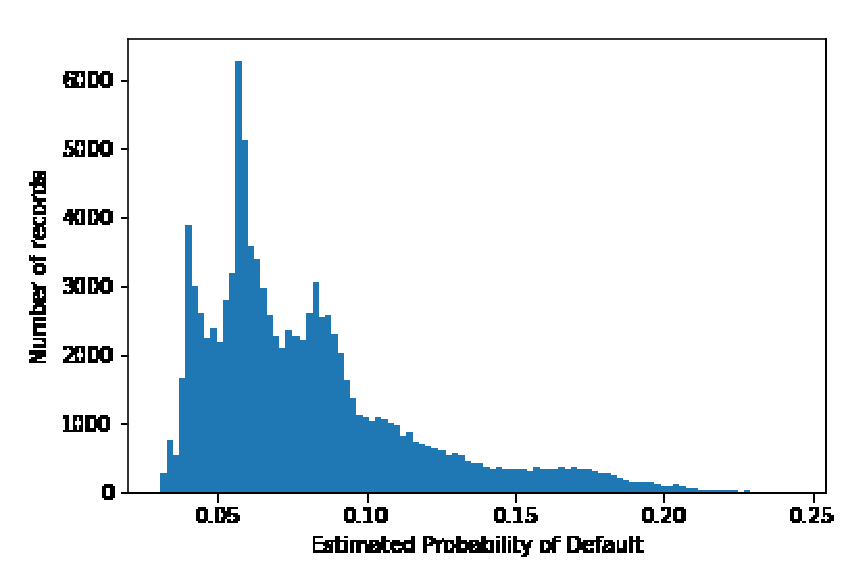
\includegraphics[clip, scale=0.80]{./hist.eps}
  \end{center}
\end{figure}
    \begin{Shaded}
\begin{Highlighting}[]
\NormalTok{use_idx }\OperatorTok{=}\NormalTok{ np.where(ypred_old }\OperatorTok{<} \FloatTok{0.15}\NormalTok{)[}\DecValTok{0}\NormalTok{]}
\NormalTok{discard_idx }\OperatorTok{=}\NormalTok{ np.where(ypred_old }\OperatorTok{>=} \FloatTok{0.15}\NormalTok{)[}\DecValTok{0}\NormalTok{]}

\NormalTok{Xnew }\OperatorTok{=}\NormalTok{ Xfold2[use_idx, :]}
\NormalTok{ynew }\OperatorTok{=}\NormalTok{ yfold2[use_idx]}

\NormalTok{Xdiscard }\OperatorTok{=}\NormalTok{ Xfold2[discard_idx, :]}
\NormalTok{ydiscard }\OperatorTok{=}\NormalTok{ yfold2[discard_idx]}
\NormalTok{ypred_discard }\OperatorTok{=}\NormalTok{ ypred_old[discard_idx]}
\end{Highlighting}
\end{Shaded}

    今回は閾値を0.15として計算した。

    \subsubsection{Step 4 New
Model1の学習}\label{step-4-new-model1ux306eux5b66ux7fd2}

    \begin{Shaded}
\begin{Highlighting}[]
\NormalTok{new_model1 }\OperatorTok{=}\NormalTok{ RandomForestRegressor(max_depth}\OperatorTok{=}\DecValTok{5}\NormalTok{, n_estimators}\OperatorTok{=}\DecValTok{100}\NormalTok{, n_jobs}\OperatorTok{=-}\DecValTok{1}\NormalTok{)}
\NormalTok{new_model1.fit(Xnew, ynew)}
\end{Highlighting}
\end{Shaded}

    \subsubsection{Step 5-7 データセット作成\textasciitilde{}New
Model2学習}\label{step-5-7-ux30c7ux30fcux30bfux30bbux30c3ux30c8ux4f5cux6210new-model2ux5b66ux7fd2}

    \begin{Shaded}
\begin{Highlighting}[]
\KeywordTok{class}\NormalTok{ SamplingRegressor:}
    \KeywordTok{def} \FunctionTok{__init__}\NormalTok{(}\VariableTok{self}\NormalTok{, data, ypred, base_estimator, nsample}\OperatorTok{=}\DecValTok{200}\NormalTok{):}
        \VariableTok{self}\NormalTok{.nsample }\OperatorTok{=}\NormalTok{ nsample}
        \VariableTok{self}\NormalTok{.clfs }\OperatorTok{=}\NormalTok{ [base_estimator }\ControlFlowTok{for}\NormalTok{ i }\KeywordTok{in} \BuiltInTok{range}\NormalTok{(nsample)]}
        \VariableTok{self}\NormalTok{.discarded }\OperatorTok{=}\NormalTok{ data}
        \VariableTok{self}\NormalTok{.samples }\OperatorTok{=}\NormalTok{ [random.binomial(}\DecValTok{1}\NormalTok{, ypred) }\ControlFlowTok{for}\NormalTok{ i }\KeywordTok{in} \BuiltInTok{range}\NormalTok{(nsample)]}
        \VariableTok{self}\NormalTok{.X }\OperatorTok{=} \VariableTok{None}
        \VariableTok{self}\NormalTok{.y }\OperatorTok{=}\NormalTok{ []}
        
    \KeywordTok{def}\NormalTok{ fit(}\VariableTok{self}\NormalTok{, X, y):}
        \VariableTok{self}\NormalTok{.X }\OperatorTok{=}\NormalTok{ np.vstack([X, }\VariableTok{self}\NormalTok{.discarded])}
        \VariableTok{self}\NormalTok{.y }\OperatorTok{=}\NormalTok{ [np.hstack([y, s]) }\ControlFlowTok{for}\NormalTok{ s }\KeywordTok{in} \VariableTok{self}\NormalTok{.samples]}
        \ControlFlowTok{for}\NormalTok{ i, clf }\KeywordTok{in} \BuiltInTok{enumerate}\NormalTok{(}\VariableTok{self}\NormalTok{.clfs):}
\NormalTok{            clf.fit(}\VariableTok{self}\NormalTok{.X, }\VariableTok{self}\NormalTok{.y[i])}
\NormalTok{            percentage }\OperatorTok{=}\NormalTok{ (i}\OperatorTok{+}\DecValTok{1}\NormalTok{) }\OperatorTok{/} \VariableTok{self}\NormalTok{.nsample }\OperatorTok{*} \DecValTok{100}
\NormalTok{            sys.stdout.write(}\SpecialStringTok{f"}\CharTok{\textbackslash{}r}\SpecialCharTok{\{}\NormalTok{percentage}\SpecialCharTok{:.2f\}}\SpecialStringTok{ percent finished"}\NormalTok{)}
        \BuiltInTok{print}\NormalTok{()}
            
    \KeywordTok{def}\NormalTok{ predict(}\VariableTok{self}\NormalTok{, X):}
\NormalTok{        preds }\OperatorTok{=}\NormalTok{ np.zeros(X.shape[}\DecValTok{0}\NormalTok{])}
        \ControlFlowTok{for}\NormalTok{ clf }\KeywordTok{in} \VariableTok{self}\NormalTok{.clfs:}
\NormalTok{            preds }\OperatorTok{+=}\NormalTok{ clf.predict(X)}
        \ControlFlowTok{return}\NormalTok{ preds }\OperatorTok{/} \VariableTok{self}\NormalTok{.nsample}
    
\NormalTok{rf }\OperatorTok{=}\NormalTok{ RandomForestRegressor(max_depth}\OperatorTok{=}\DecValTok{5}\NormalTok{, n_estimators}\OperatorTok{=}\DecValTok{100}\NormalTok{, n_jobs}\OperatorTok{=-}\DecValTok{1}\NormalTok{)}
\NormalTok{new_model2 }\OperatorTok{=}\NormalTok{ SamplingRegressor(Xdiscard, ypred_discard, rf, }\DecValTok{1000}\NormalTok{)}
\NormalTok{new_model2.fit(Xnew, ynew)}
\end{Highlighting}
\end{Shaded}

    \subsubsection{Step 8 検証}\label{step-8-ux691cux8a3c}

    \begin{Shaded}
\begin{Highlighting}[]
\NormalTok{validation_model }\OperatorTok{=}\NormalTok{ RandomForestRegressor(max_depth}\OperatorTok{=}\DecValTok{5}\NormalTok{, n_estimators}\OperatorTok{=}\DecValTok{100}\NormalTok{, n_jobs}\OperatorTok{=-}\DecValTok{1}\NormalTok{)}
\NormalTok{validation_model.fit(Xfold2, yfold2)}

\NormalTok{pred1 }\OperatorTok{=}\NormalTok{ new_model1.predict(Xfold3)}
\NormalTok{pred2 }\OperatorTok{=}\NormalTok{ new_model2.predict(Xfold3)}
\NormalTok{pred3 }\OperatorTok{=}\NormalTok{ validation_model.predict(Xfold3)}

\NormalTok{idx }\OperatorTok{=}\NormalTok{ np.where(pred3 }\OperatorTok{-}\NormalTok{ pred1 }\OperatorTok{>} \FloatTok{0.1}\NormalTok{)[}\DecValTok{0}\NormalTok{]}
\BuiltInTok{print}\NormalTok{((pred2[idx] }\OperatorTok{>} \FloatTok{0.15}\NormalTok{).mean())}
\end{Highlighting}
\end{Shaded}

    これによりOld Modelでは審査落ちしていてNew
Model1ではPDが低く出ていたデータのうち \textbf{98.8\%}
が提案手法ではPDが高い(閾値以上)と予測されることがわかった。

    なお、確認のためROC曲線を描いてみたのが以下の図\label{fig:roc}である。
\begin{figure}[htbp]
  \begin{center}
    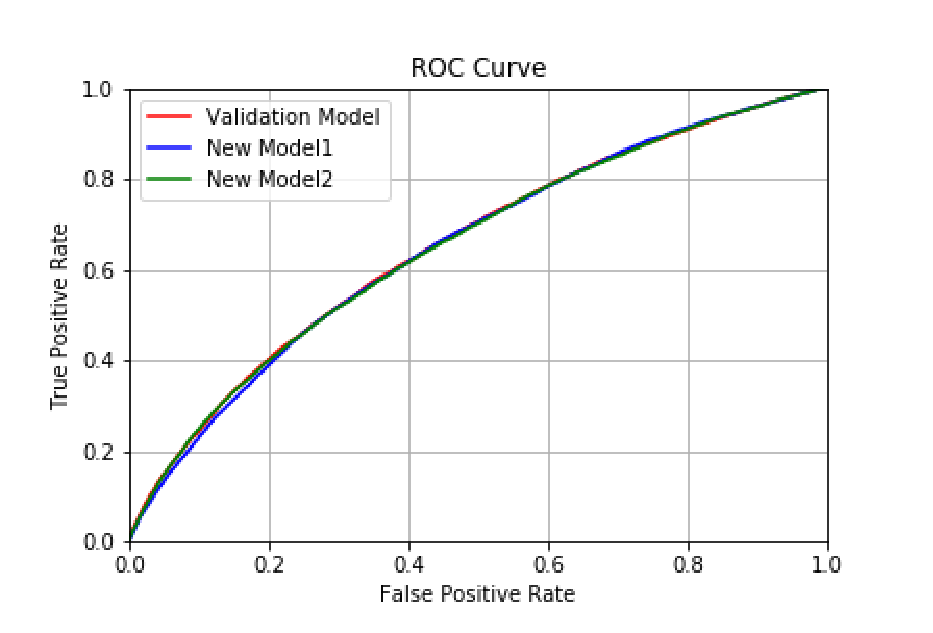
\includegraphics[clip, scale=0.80]{./ROC_CURVE.eps}
    \label{fig:roc}
  \end{center}
\end{figure}
    AUCでは、Validation Modelが0.653, New Model1が0.649, New
Model2が0.651となった。

    \section{価値提案}\label{ux4fa1ux5024ux63d0ux6848}

    最後に提案したモデルについて、価格設定を行う。本モデルには \textbf{\$
40,000} の価格を設定する。この価格の根拠は以下のとおりである。

    まず、Home Credit
GroupがHome-Credit-Default-Riskのコンペティションに設定した賞金は総額\$
70,000であり、一位の賞金は\$
35,000である。この価格設定は、コンペティションに対してHome Credit
Groupがかけている期待を反映したものであると言える。先に述べたとおり、Home
Credit Groupがこのコンペティションに求めているものは、Home Credit
Groupが抱えている課題を解決するデータ分析のやり方のヒントであって提出されるモデルそのものではない。すなわち、実務に直接使えるものではなく、その業務を改善するヒントに
\$
70,000という額を設定していると考えられる。これは将来にわたってのクレジットスコアリングモデル構築費用の一部の額を積分した値と捉えることができる。

また、同業である富士通総研ではクレジットスコアリングモデル構築に\$
50,000以上という価格設定をしている\cite{fujitsu}。これを考えて、クレジットスコアリングモデルの相場はおよそ\$
30,000 - \$
100,000程度であると予測した。この上で今回のスコアリングモデルはHome
Credit
Groupが抱える課題にクリティカルに作用する解決策を含むもののその他の部分での手法的目新しさはなく、運用中に改善を多く施すことになると考えられることから、スコアリングモデルの価格の下限に近い\$
40,000を設定した。


    % Add a bibliography block to the postdoc
    
    
    \bibliographystyle{junsrt}
    \bibliography{reference}
    
    
    \end{document}
